
\section{System Block Division}
\begin{frame}[c] \frametitle{System Block Division}
The modules which defines the defines the demodulator.
    \begin{figure}[htbp]
        \centering
        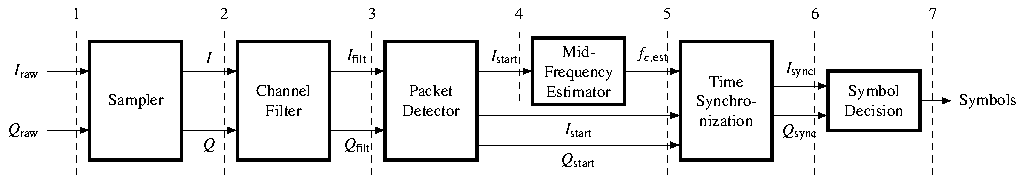
\includegraphics[width=1\textwidth]{img/interfaces}
    \end{figure}
\end{frame}


\subsection{Sampler} \label{sec:sampler}

\begin{frame} \frametitle{Sampler}
    \framesubtitle{Sorting Data Input}
Sorting the input data.
    \begin{center}
        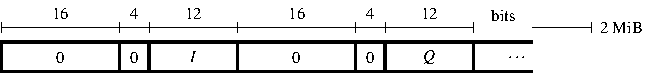
\includegraphics[width=1\textwidth]{img/sampler1}
    \end{center}





    \begin{center}
        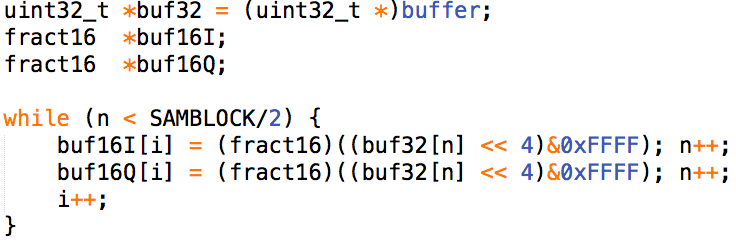
\includegraphics[width=0.8\textwidth]{img/sampler_snippet}
    \end{center}
    \begin{itemize}
        \item Implementation appropriate inside the channel filter.
    \end{itemize}
\end{frame}


\subsection{Channel Filter} \label{sec:filter}

\begin{frame} \frametitle{Channel Filter}
    \framesubtitle{Choices}
    \begin{center}
        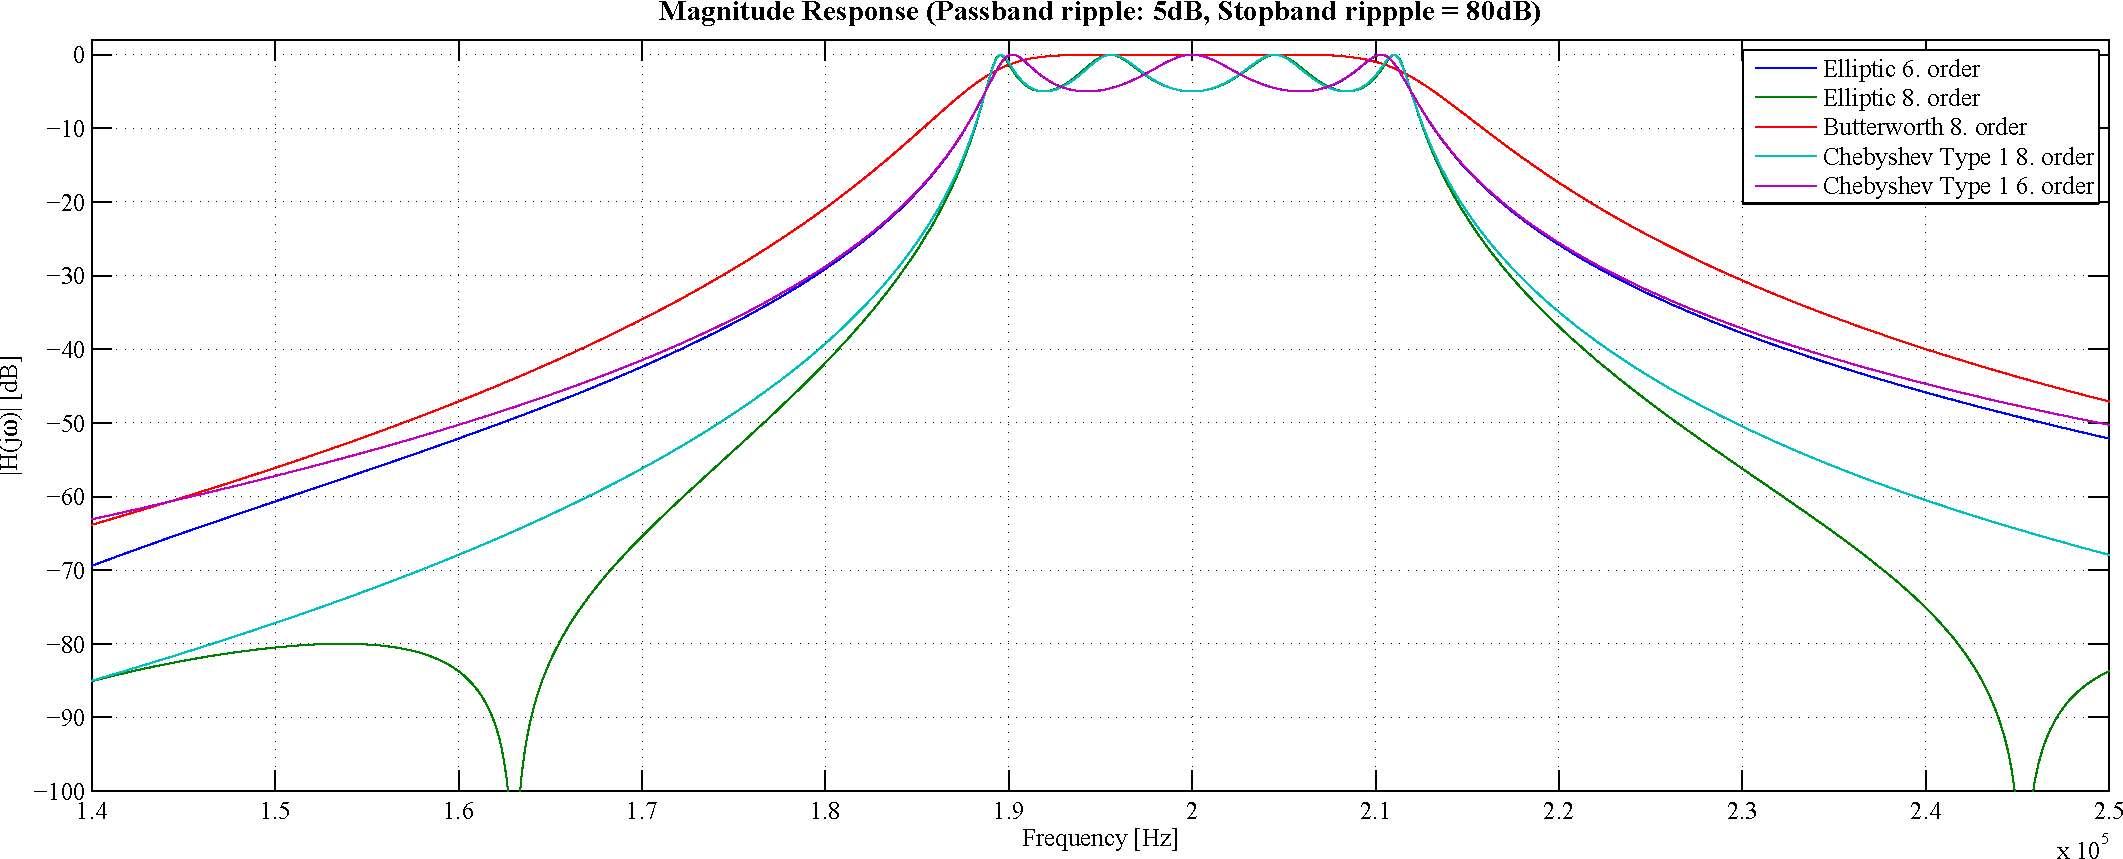
\includegraphics[width=1\textwidth]{img/filter2_frq_res}
    \end{center}
    \begin{itemize}
        \item Bandwidth is defined from Doppler range.
        \item Frequency characteristic is chosen from existing filter
        \item Group Delay of Butterworth is constant.
    \end{itemize}
\end{frame}


\begin{frame} \frametitle{Channel Filter}
    \framesubtitle{Design}
%
% Equation of Bandpass transformation 
%    
    \begin{itemize}
        \item 4th order LP $\rightarrow$ 8th order BP.
    \end{itemize}
\begin{equation*}
    \begin{aligned}
        H(s) &= \left.\frac{1}{s^4 + 2.61s^3 + 3.41s^2 + 2.61s + 1} \right|_{s = \frac{S^2 + \Omega_0^2}{B S}}\\
    \end{aligned}
\end{equation*}


%
% Equation of Bilinear Done 
%    
\begin{equation*}
    \begin{aligned}
    \left. H(z) = \frac{B^4 S^4 }{a S^8 + b S^7 + c S^6 + d S^5 + e S^4 + f S^3 + g S^2 + h S + i}\right|_{S  = \frac{2}{T_S}\cdot\frac{z-1}{z+1}}\\
\label{eq:bilinear_done}
\end{aligned}
\end{equation*}
    \begin{itemize}
    \item[a] $= 1$
    \item[b] $= 2.61B$
    \item[c] $= 3.41B^2 + 4\Omega_\text{0}^2$
    \item[d] $= 2.61B(B^2 + 3\Omega_\text{0}^2)$
    \item[e] $= B^4 + 6.82B^2 \Omega_\text{0}^2 + 6\Omega_\text{0}^4$
    \item[f] $= 2.61B(B^2 + 3\Omega_\text{0}^2)\Omega_\text{0}^2$     
    \item[g] $= 3.41 B^2 \Omega_\text{0}^4 + 4\Omega_\text{0}^6$ 
    \item[h] $= 2.61 B \Omega_\text{0}^6$
    \item[i] $= \Omega_\text{0}^8$
    \end{itemize}
\end{frame}



\begin{frame} \frametitle{Channel Filter}
    \framesubtitle{Implementation}

\begin{equation*}
\resizebox{9cm}{!}{
        % \begin{aligned}
    $H(z) = 67.263\text{E-6} \cdot \frac{1 - 4z^{-2} + 6z^{-4} - 4z^{-6} + z^{-8} }{1 + 0.65 z^{-1} + 3.65 z^{-2} + 1.73 z^{-3} + 4.89 z^{-4} + 1.52 z^{-5} + 2.84 z^{-6} + 0.44 z^{-7} + 0.60z^{-8}}$
    % \label{eq:chan_filt_bp_filter}
% \end{aligned}
}
\end{equation*}
\begin{itemize}
    \item 2nd order cascades by pairing poles closest to unit circle with the closest zero.
\end{itemize}
\begin{equation*}
    H(z) = k\cdot\frac{(z-z_1)(z-z_2)}{(z-p_n)(z-p_n^*)}\quad=\quad k\cdot\frac{b_0+b_1z^{-1}+b_2z^{-2}}{a_0+a_1z^{-1}+a_2z^{-2}}
\end{equation*}
\begin{itemize}
    \item Discrete Time Domain
\end{itemize}
\begin{equation*}
           y(n) = b_0x(n) + b_1x(n-1) + b_2x(n-2) - a_1y(n-1) - a_2y(n-2)
\end{equation*}
\end{frame}

\begin{frame} \frametitle{Channel Filter}
        \framesubtitle{Cascade Form}
Direct Form II
    \begin{center}
        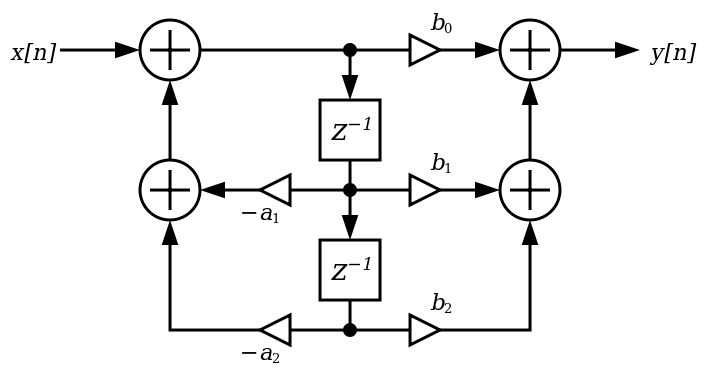
\includegraphics[scale=0.3]{img/biquadDF2}
    \end{center}

\begin{equation*}
        \begin{aligned}
    w(n) &= x(n)     - a_1 w(n-1) - a_2 w(n-2)   \\
    y(n) &= b_0 w(n) + b_1 w(n-1) + b_2 w(n-2)
    \label{eq:df2}
\end{aligned}
\end{equation*}
\end{frame}
% To reduce the sensitivity of coefficient quantisation, the filter is implemented in a cascade structure consisting of second order sections \cite[page 153]{kuo2007real}. With cascade form, variations in one parameter only affects the related section, where variations in direct form parameters influence all the poles. Therefore cascaded form is preferred in DSP implementation, especially for higher order filters. Each section generates roundoff error, which is propagated to the next stage. The total roundoff noise will depend on the specific ordering and pairing of poles. 
% To prevent overflow either scale factors or another Q format with higher dynamic range can be applied. Scale factors can be used at each section to avoid overflow, at the cost of lower SNR. %\cite[page 158]{kuo2007real}. 


\begin{frame} \frametitle{Channel Filter}
    \framesubtitle{Implementation}
    \begin{center}
        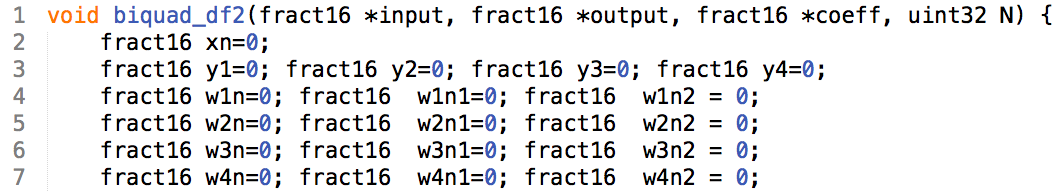
\includegraphics[width=0.8\textwidth]{img/filter_snippet}
    \end{center}
    \begin{center}
        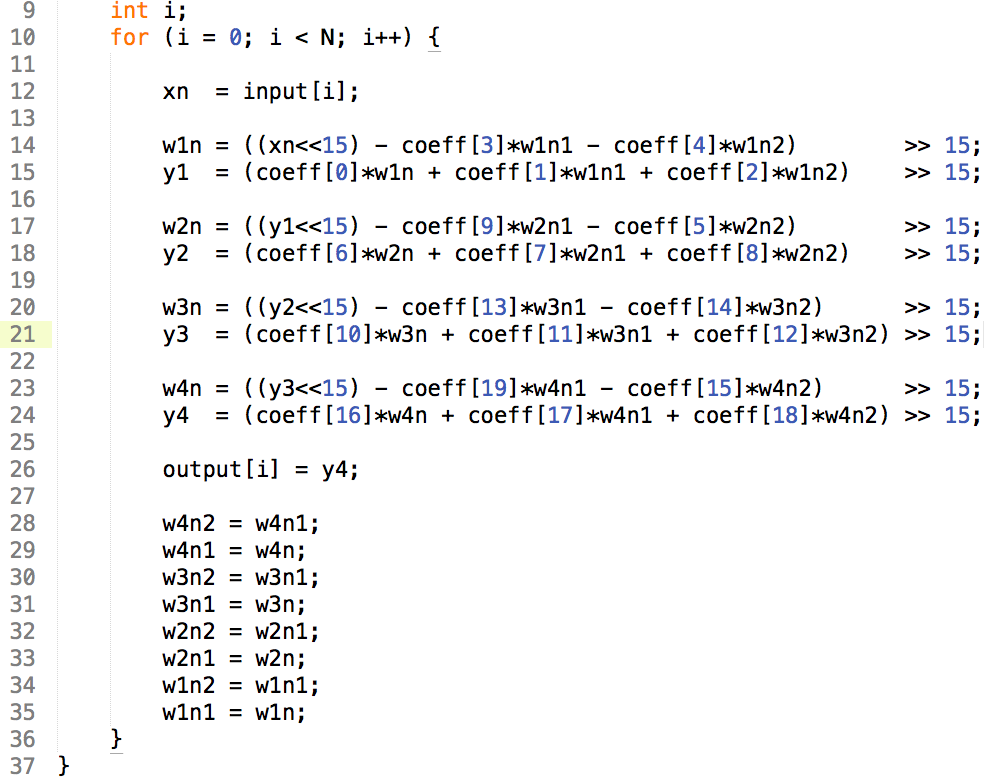
\includegraphics[width=0.8\textwidth]{img/filter_loop}
    \end{center}
\end{frame}

\begin{frame} \frametitle{Channel Filter}
    \framesubtitle{Implementation}
    \begin{itemize}
        \item C-Code
    \end{itemize}
    \begin{center}
        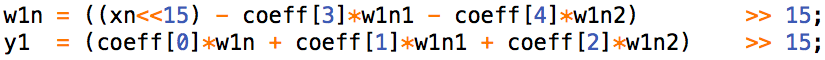
\includegraphics[width=0.8\textwidth]{img/filter_C_cascade}
    \end{center}
    \begin{itemize}
        \item Assembly
    \end{itemize}
    \begin{center}
        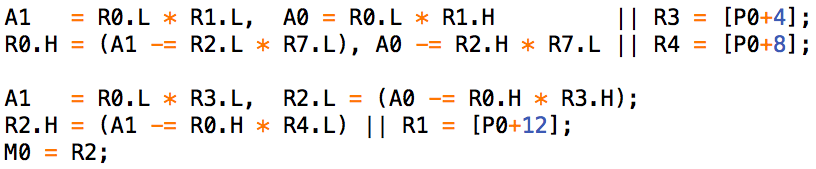
\includegraphics[width=0.8\textwidth]{img/filter_asm_cascade}
    \end{center}
\end{frame}
% \begin{frame} \frametitle{Channel Filter}
%     \framesubtitle{Results}
%     \begin{center}
%         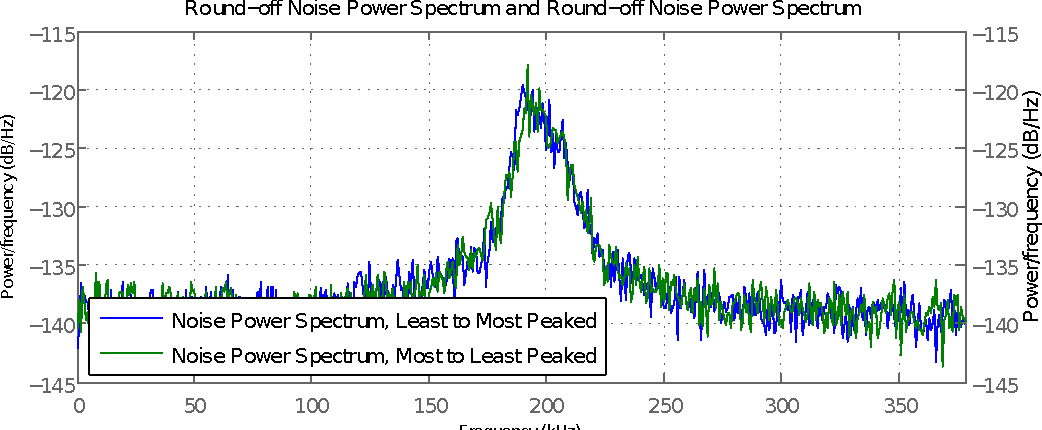
\includegraphics[scale=0.5]{img/filter6_noise}
%     \end{center}
% \end{frame}

\begin{frame} \frametitle{Channel Filter}
    \framesubtitle{Test on Blackfin DSP}
DSP test with Q15 frequency sweep and C-filter
    \begin{center}
        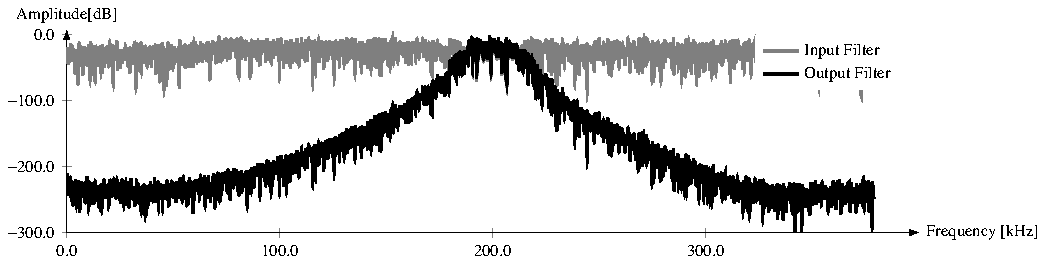
\includegraphics[width=\textwidth]{img/filter7_test_freq_res}
    \end{center}
\begin{itemize}
    \item Frequency Characteristic as specified.
    \item Theoretical cycle usage of $1.8\%$ (Optimal)
\end{itemize}
%     \begin{center}
%         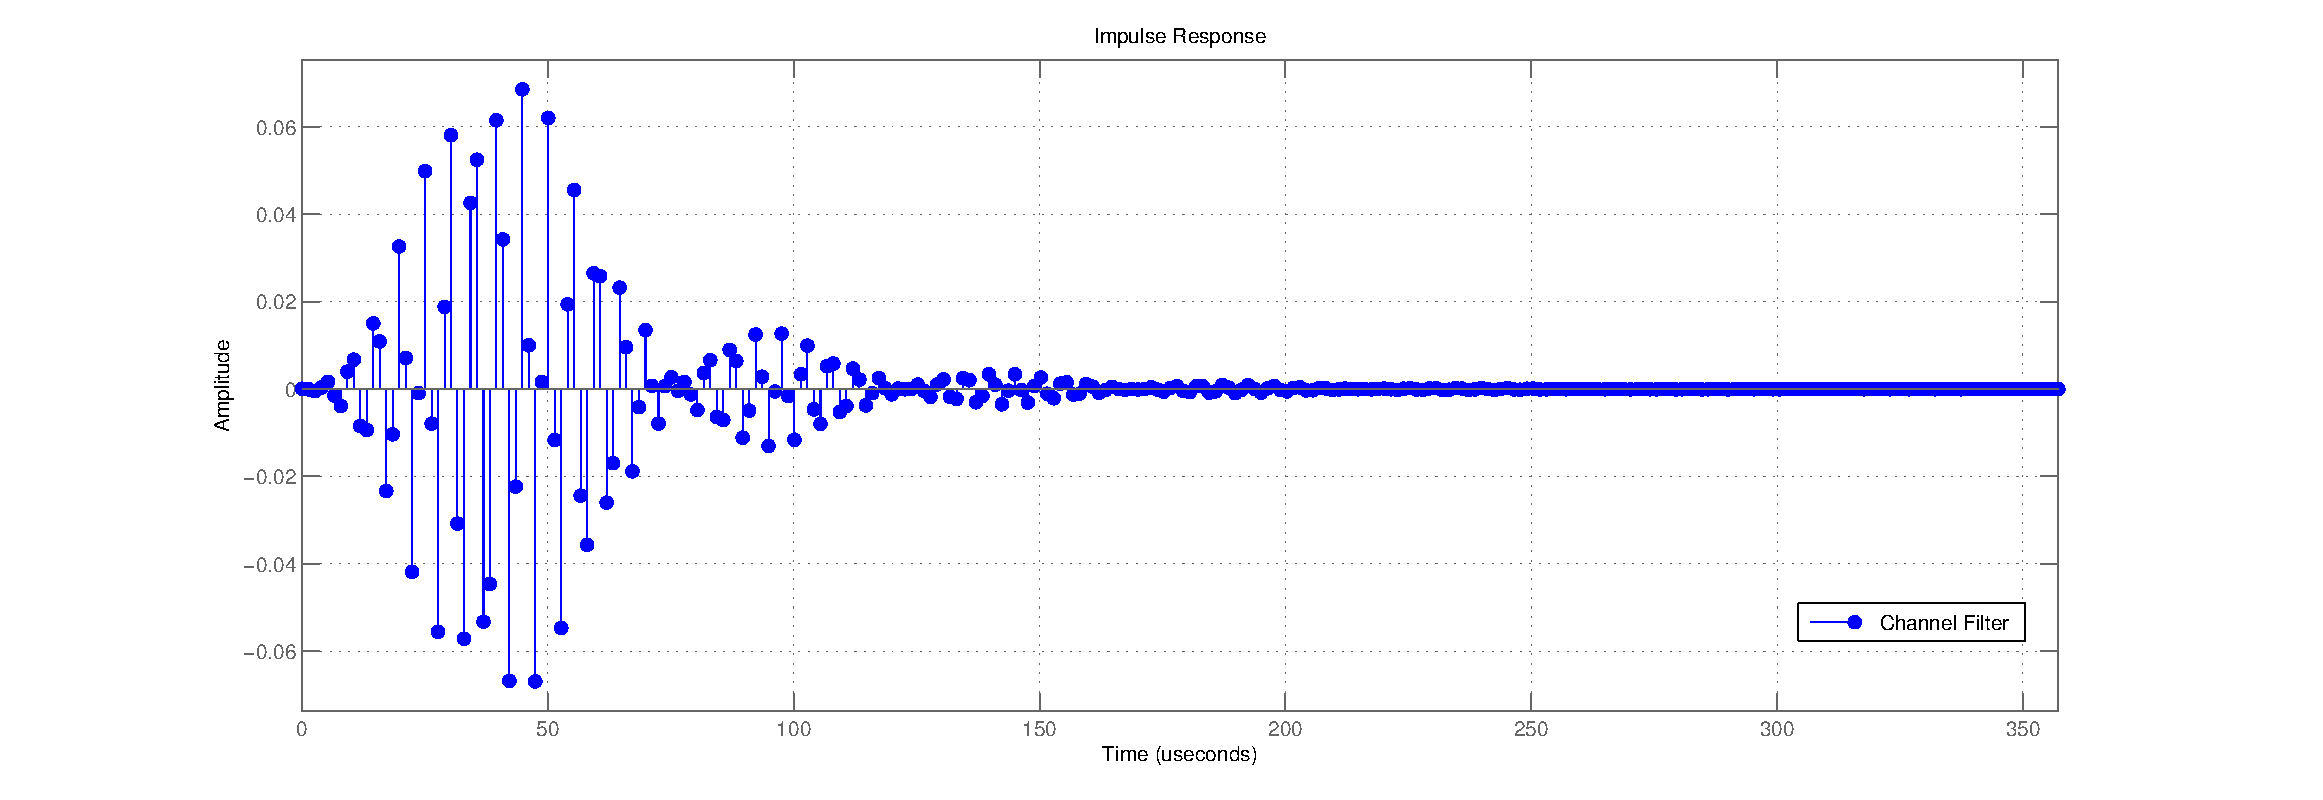
\includegraphics[scale=0.2]{img/filter5_imp_res}
%     \end{center}
\end{frame}

\subsection{Packet Detection}
\begin{frame} \frametitle{Packet Detection}
    \framesubtitle{Double Sliding Window Design}
        \begin{equation*}
            E_w(n) = \frac{1}{N}\sum_{i=n-N+1}^{n} x_i^2
        \end{equation*}
        \begin{equation*}
            Ratio(n) = \frac{E_w(n)}{E_w(n-N)} 
        \end{equation*}
    \begin{center}
        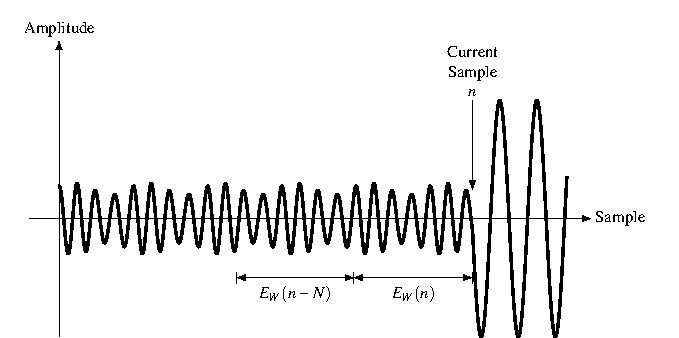
\includegraphics[width=\textwidth]{img/dsw4}
    \end{center}

\end{frame}


\begin{frame} \frametitle{Packet Detection}
    \framesubtitle{Test of Window Size at \SI{5}{dB} SNR}
 
    \begin{center}
        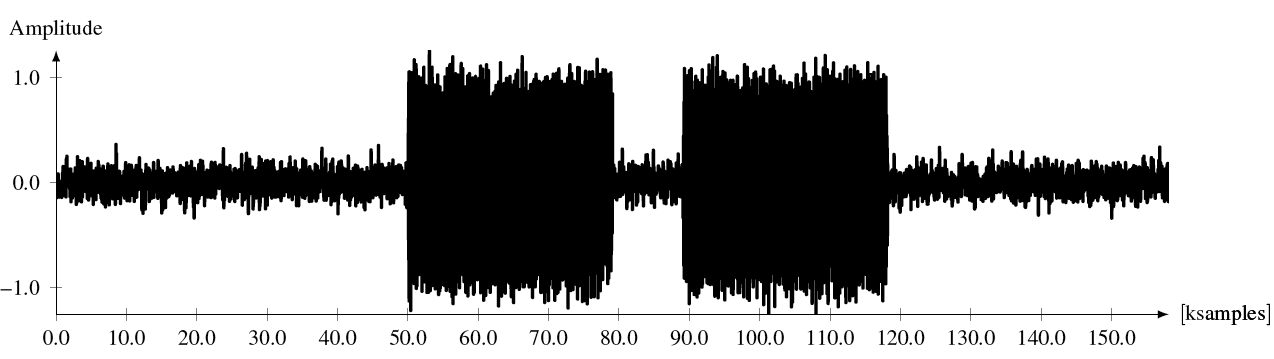
\includegraphics[width=\textwidth]{img/dsw3}
    \end{center}

    \begin{center}
        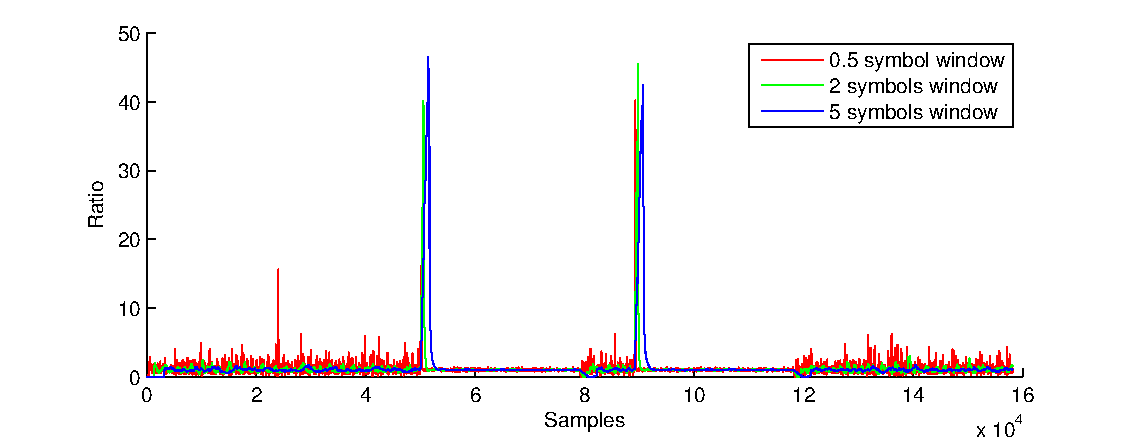
\includegraphics[width=\textwidth]{img/dsw6}
    \end{center}
\end{frame}


\begin{frame} \frametitle{Packet Detection}
    \framesubtitle{Test of SNR Influence with Window Size of 2 Symbols}
    
    % \begin{center}
    %     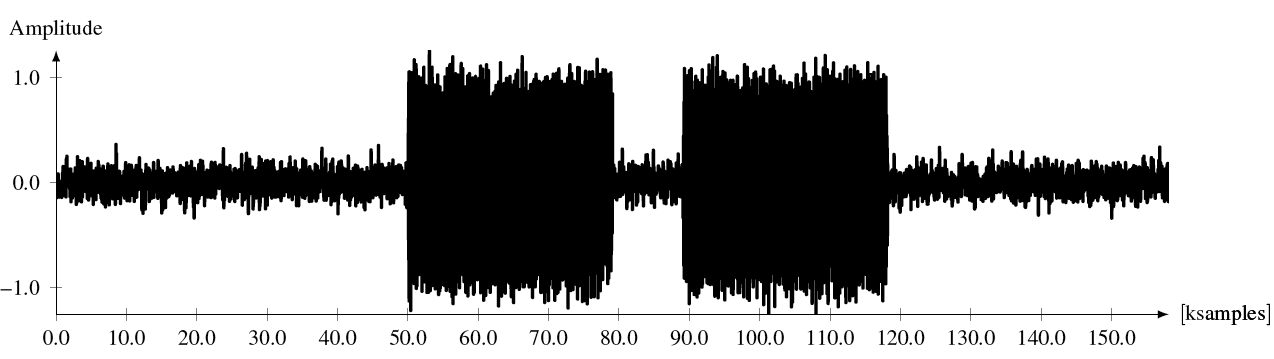
\includegraphics[width=\textwidth]{img/dsw3}
    % \end{center}V
    \begin{equation*}
        W_{model} \approx \mathcal{N}(\mu,\sigma^2) , \mu=0
    \end{equation*}    
    \begin{equation*}
        P_n = \sigma^2 = \frac{P_s}{SNR}
    \end{equation*}    
    \begin{center}
        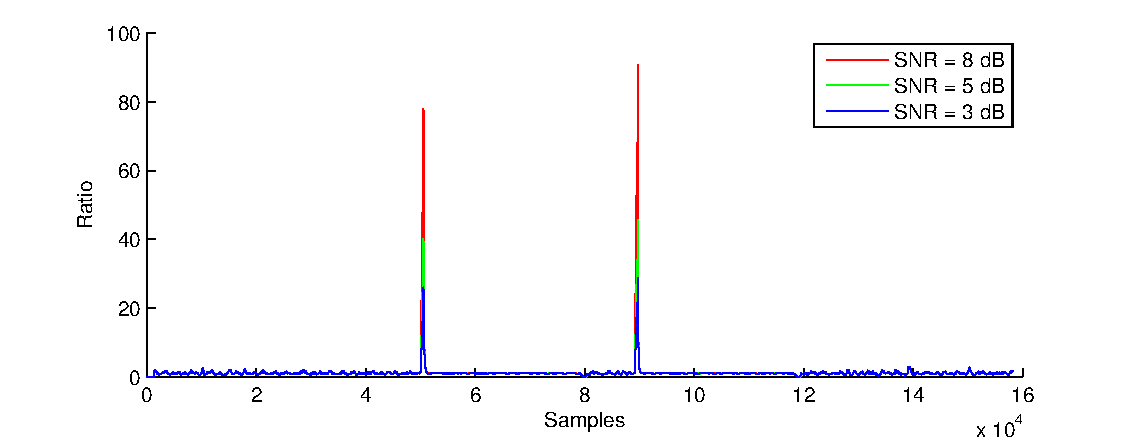
\includegraphics[width=\textwidth]{img/dsw5}
    \end{center}

\end{frame}

\begin{frame} \frametitle{Packet Detection}
    \framesubtitle{Implementation}
    \begin{equation*}
        E_w(n) = E_w(n) - \frac{x_{n-N}^2}{N} + \frac{x_n^2}{N}
    \end{equation*}
    \begin{center}
        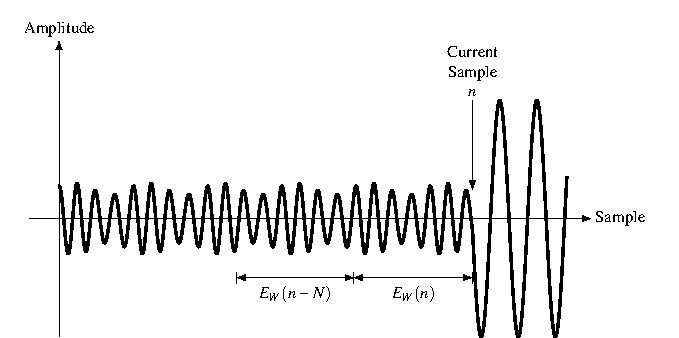
\includegraphics[width=0.8\textwidth]{img/dsw4}
    \end{center}
    \begin{itemize}
        \item Window size power of two.
        \item Store old windows as a constant vector
        \item 2 mult, 1 sub, 1 add, 1 division
    \end{itemize}
\end{frame}
